\documentclass[12pt]{article}
\usepackage[utf8]{inputenc}
\usepackage{graphicx} % Per includere immagini
\usepackage{titling}  % Per personalizzare lo spazio del titolo
\usepackage{ccicons}  % Per i simboli Creative Commons
\usepackage{geometry} % Per personalizzare i margini
\usepackage{hyperref} % Per i link
\usepackage[italian]{babel}
\usepackage{pgffor}
\usepackage{listings}
\usepackage{color}

\definecolor{codegreen}{rgb}{0,0.6,0}
\definecolor{codegray}{rgb}{0.5,0.5,0.5}
\definecolor{codepurple}{rgb}{0.58,0,0.82}
\definecolor{backcolour}{rgb}{0.95,0.95,0.92}

\lstdefinestyle{mystyle}{
    backgroundcolor=\color{backcolour},   
    commentstyle=\color{codegreen},
    keywordstyle=\color{magenta},
    numberstyle=\tiny\color{codegray},
    stringstyle=\color{codepurple},
    basicstyle=\ttfamily\footnotesize,
    breakatwhitespace=false,         
    breaklines=true,                 
    captionpos=b,                    
    keepspaces=true,                 
    numbers=left,                    
    numbersep=5pt,                  
    showspaces=false,                
    showstringspaces=false,
    showtabs=false,                  
    tabsize=2
}

\lstset{style=mystyle}

% Imposta i margini della pagina
\geometry{
  top=2cm,
  bottom=2cm,
  left=3cm,
  right=3cm
}

\lstset{
  basicstyle=\ttfamily,
  breaklines=true,
  columns=fullflexible
}

\setlength{\droptitle}{-5em} % Sposta in alto il titolo

\title{
    \Large \textbf{UNIVERSITA' DI SALERNO} \\[0.5em]
    \small DIPARTIMENTO DI INGEGNERIA DELL'INFORMAZIONE ED ELETTRICA E MATEMATICA APPLICATA\\[5em]
    
\includegraphics[width=0.6\textwidth]{logo_uni.png}\\[3em] % Logo dell'Università
    \normalsize Laurea Magistrale in Ingegneria Informatica \\[1em]
    \Large \textbf {Project work} \\[1em]
    \large \textbf {Deliverable 1} \\ [1em]
    \large {Sistemi Embedded} \\[1em]
}

\author{
    \textbf{Gruppo: 8} \\
    \normalsize Marotta Giuseppe - 0622702302 - g.marotta@studenti.unisa.it\\
    \normalsize Rea Gaetano - 0622702190 - g.rea7@studenti.unisa.it\\
    \normalsize Squitieri Giuseppe - 0622702339 - g.squitieri8@studenti.unisa.it\\ 
    \normalsize Tramice Davide - 0622702194 - d.tramice@studenti.unisa.it\\ \\
    }

\date{
    ANNO ACCADEMICO 2023/2024 % Data
}

\begin{document}

\begin{titlingpage} % Crea una pagina di titolo personalizzata
\maketitle
\thispagestyle{empty} % Rimuove il numero di pagina
%\begin{center}
    %\ccbyncnd % Simbolo Creative Commons
%\end{center}
\end{titlingpage}

% Creazione di una nuova pagina
\newpage

% Aggiungi l'indice delle sezioni
\tableofcontents

\newpage

\section{Progettazione del sistema}

Questa sezione approfondisce la metodologia di progettazione adottata per sviluppare il sistema, delineando i processi, le strategie e gli approcci utilizzati per garantire un'architettura robusta e un funzionamento ottimale. \\\\
In questa fase di progettazione, vengono utilizzati diversi diagrammi UML (Unified Modeling Language) per fornire una rappresentazione visuale dell'architettura e del funzionamento del sistema. Questi diagrammi sono strumenti essenziali per comunicare in modo chiaro e conciso la struttura 
e le interazioni all'interno del sistema.
\\\\
Attraverso l'analisi dettagliata della progettazione, si mira a garantire che il sistema soddisfi appieno le esigenze degli utenti e che sia in grado di fornire le funzionalità desiderate in modo efficiente, sicuro e affidabile.
\subsection{User stories}
Le user stories rappresentano una componente essenziale della fase di progettazione, fornendo una panoramica diretta e comprensibile delle funzionalità richieste dal punto di vista dell'utente. 
\\\\
Queste narrazioni brevi sono strumenti efficaci per catturare le esigenze degli utenti finali e guidare lo sviluppo del sistema in modo centrato sull'utente. Ogni user story è accompagnata da criteri di accettazione chiari e obiettivi, che stabiliscono in modo inequivocabile quando una determinata funzionalità può essere considerata completa e soddisfacente per l'utente. 
\\\\
Questo approccio aiuta a garantire che il processo di progettazione si concentri sulle reali esigenze degli utenti e fornisce un solido punto di riferimento per la fase di testing, consentendo di valutare in modo efficace il grado di conformità del sistema alle aspettative degli utenti finali.
\subsubsection{US1: Apertura cancello}
Come utente, \\
voglio essere in grado di aprire il cancello quando è chiuso o in fase di chiusura premendo il pulsante B1, \\
in modo tale da pote entrare.
\begin{itemize}
    \item Criterio di accettazione
    \begin{enumerate}
        \item Quando l'utente preme il pulsante B1 e il cancello è chiuso quest'ultimo va in fase di apertura.
        \item Quando l'utente preme il pulsante B1 e il cancello è in fase di chiusura quest'ultimo va in fase di apertura.
        \item Quando il cancello è in fase di apertura il led giallo lampeggia con una frequenza di 0.5Hz, dopo la fase di apertura tutti i led sono accesi.
    \end{enumerate}
\end{itemize}
\subsubsection{US2: Chiusura cancello}
Come utente, \\
voglio essere in grado di chiudere il cancello quando è aperto o in fase di apertura premendo il pulsante B1, \\
in modo tale da poter chiudere la casa.
\begin{itemize}
    \item Criterio di accettazione
    \begin{enumerate}
        \item Quando l'utente preme il pulsante B1 e il cancello è aperto quest'ultimo va in fase di chiusura.
        \item Quando l'utente preme il pulsante B1 e il cancello è in fase di apertura quest'ultimo va in fase di chiusura.
        \item Quando il cancello è in fase di chiusura il led giallo lampeggia con una frequenza di 0.5Hz, dopo la fase di chiusura tutti i led spenti.
    \end{enumerate}
\end{itemize}
\subsubsection{US3: Regolazione tempo di chiusura}
Come utente, \\
voglio poter regolare, premendo il pulsante B2, il tempo di chiusura automatica del cancello,\\
in modo tale che quando passa il tempo che ho scelto il cancello si chiude quando è aperto.
\begin{itemize}
    \item Criteri di accettazione
    \begin{enumerate}
        \item Premere il pulsante B2 aumenta il tempo di chiusura automatica del cancello.
        \item Il tempo di chiusura automatica varia da 10 a 120 secondi.
        \item Quando il tempo massimo (120 secondi) è raggiunto e si preme nuovamente il pulsante B2, il tempo ritorna a 10 secondi.
    \end{enumerate}
\end{itemize}
\subsubsection{US4: Regolazione tempo di lavoro}
Come utente, \\
voglio poter regolare, premendo il pulsante B3, il tempo di lavoro del cancello,\\
in modo tale da decidere la durata della fase di chiusura e apertura.
\begin{itemize}
    \item Criteri di accettazione
    \begin{enumerate}
        \item Premere il pulsante B3 aumenta il tempo di lavoro del cancello.
        \item Il tempo di lavoro varia da 10 a 120 secondi.
        \item Quando il tempo massimo (120 secondi) è raggiunto e si preme nuovamente il pulsante B3, il tempo ritorna a 10 secondi.
    \end{enumerate}
\end{itemize}
\subsubsection{US5: Riapertura ostacolo}
Come utente, \\
voglio che il cancello si riapra se viene rilevata la presenza dal sensore P1 di un ostacolo durante la fase di chiusura,\\
in modo tale da non provocare nessun danno.
\begin{itemize}
    \item Criteri di accettazione
    \begin{enumerate}
        \item Se il sensore P1 rileva un ostacolo durante la chiusura del cancello, il cancello ritorna in fase di apertura.
    \end{enumerate}
\end{itemize}
\subsubsection{US6: Ingora comando ostacolo}
Come utente, \\
voglio che il cancello non si apra o si chiuda se il sensore di presenza P1 rileva la presenza di un ostacolo e premo il pulsante B1,\\
in modo tale da non provocare nessun danno.
\begin{itemize}
    \item Criteri di accettazione
    \begin{enumerate}
        \item Se il sensore P1 rileva un ostacolo durante la richiesta di apertura o chiusura del cancello, il comando viene ignorato.
        \item Il led verde lampeggia per 30 secondi con frequenza di 1Hz quando il pulsante B1 viene premuto
   \end{enumerate}
\end{itemize}
\subsubsection{US7: Stato di errore sensore P2}
Come utente, \\
voglio che il cancello entri in uno stato di errore se il sensore di chiusura P2 non si attiva entro 10 secondi dopo il tempo di lavoro del cancello che è in fase di chiusura,\\
in modo tale da sapere che il cancello non rimanga aperto.
\begin{itemize}
    \item Criteri di accettazione
    \begin{enumerate}
        \item Il led rosso segnale stato di errore accendendosi se il sensore P2 non si attiva entro 10 secondi dopo il tempo di lavoro durante la fase di chiusura.
        \item Lo stato di errore persiste fino a quando il sensore P2 non si attiva.
    \end{enumerate}
\end{itemize}
\subsubsection{US8: Chiusura automatica}
Come utente, \\
voglio che quando il cancello è aperto e passa il tempo di chiusura, esso passa nella fase di chiusura\\
in modo tale da non dover premere il pulsante B1 per richiuderlo.
\begin{itemize}
    \item Criteri di accettazione
    \begin{enumerate}
        \item Quando il cancello è aperto e il tempo di chiusura è passato il cancello passa alla fase di chiusura.
        \item Quando il cancello è aperto e passa il tempo di chiusura il led giallo lampeggia con una frequenza di 0.5Hz segnalando la fase di chiusura.
    \end{enumerate}
\end{itemize}

\newpage



\subsection{Use case diagram}
Nel seguente capitolo esamineremo i vari casi d'uso relativi a ciascuna user story. Ogni caso d'uso rappresenta un'azione compiuta da un attore per interagire con il sistema esterno. All'interno di tali casi d'uso, troveremo l'utente 'Gennaro' che compie le azioni e il sistema, che è il cancello.

\subsubsection{Apertura cancello [US1]}
Questo caso d'uso, che modella US1, ha come attori l'utente e il cancello e descrive la situazione in cui l'utente desidera aprire il cancello, sia quando è chiuso che quando si sta chiudendo. L'apertura viene segnalata tramite l'illuminazione del relativo LED giallo. Il cancello aperto vine segnalato dagli appositi LED verde, giallo e rosso tutti accesi.
\begin{figure}[h]
    \centering
    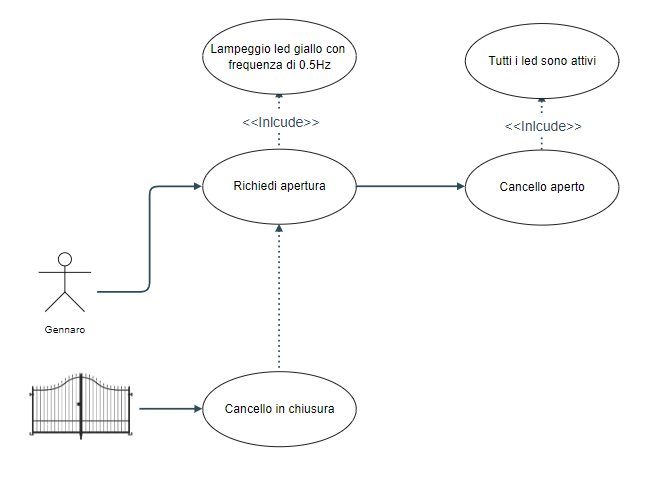
\includegraphics[width=0.6\textwidth,height=5.2cm]{use_case_us1.PNG}
    \caption{USE CASE user stories 1.}
    \label{fig:use_case_us5}
\end{figure}
\subsubsection{Chiusura cancello [US2]}
Questo caso d'uso, che modella US2, ha come attori l'utente e il cancello e descrive la situazione in cui l'utente desidera chiudere il cancello, sia quando è aperto che quando si sta aprendo. L'apertura viene segnalata tramite l'illuminazione del relativo LED giallo. Il cancello chiuso vine segnalato dagli appositi LED verde, giallo e rosso tutti spenti.
\begin{figure}[h]
    \centering
    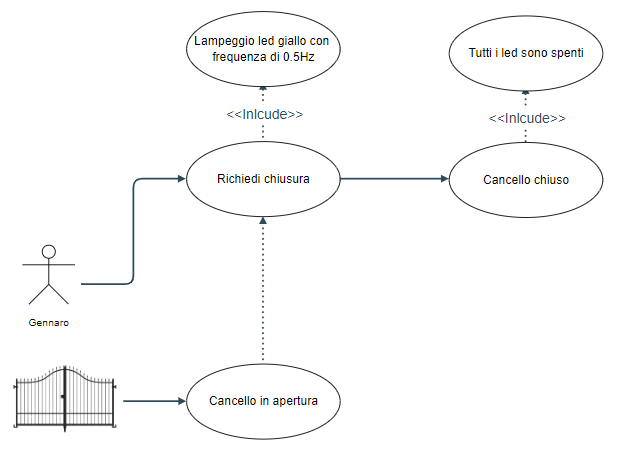
\includegraphics[width=0.6\textwidth,height=5.2cm]{use_case_us2.PNG}
    \caption{USE CASE user stories 2.}
    \label{fig:use_case_us5}
\end{figure}
\subsubsection{Regolazione tempo di chiusra [US3]}
\subsubsection{Regolazione tempo di lavoro [US5]}
\subsubsection{Riapertura ostacolo [US5]}
Questo caso d'uso, che modella US5, ha come attori l'utente e il cancello. Descrive la situazione in cui il cancello si sta chiudendo e successivamente arriva un ostacolo davanti a esso (sotto il sensore P1), causando la riapertura del cancello.
    \begin{figure}[h]
        \centering
        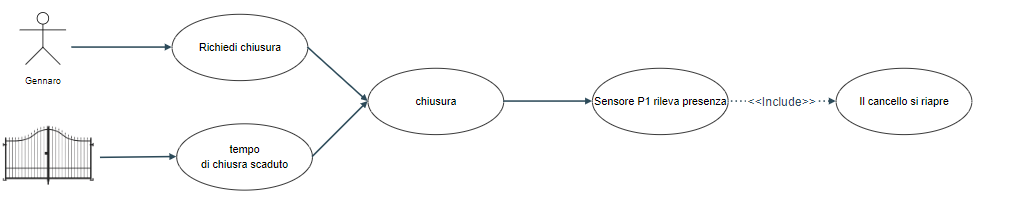
\includegraphics[width=0.8\textwidth]{use_case_us5.PNG}
        \caption{USE CASE user stories 5.}
        \label{fig:use_case_us5}
    \end{figure}
\subsubsection{Ingora comando ostacolo [US6]}
Questo caso d'uso, che modella US6, ha come attore l'utente che richiede l'apertura. Tuttavia, se è presente un ostacolo davanti al sensore P1, il comando viene ignorato. Tale situazione viene segnalata dall'attivazione del relativo LED verde per 30 secondi.
\begin{figure}[h]
    \centering
    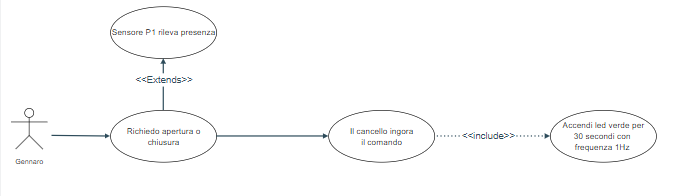
\includegraphics[width=0.8\textwidth]{use_case_us6.PNG}
    \caption{USE CASE user stories 6.}
    \label{fig:use_case_us5}
\end{figure}
\newpage
\subsubsection{Stato errore sensore P2 [US7]}
Questo caso d'uso, che modella US7, ha come attore il cancello, che entra in uno stato di allarme se non si chiude entro il tempo di lavoro più 10 secondi. La situazione di allarme viene segnalata dall'attivazione del relativo LED rosso.
\begin{figure}[h]
    \centering
    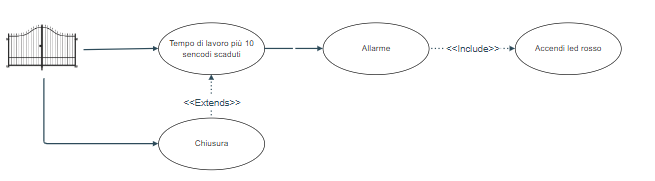
\includegraphics[width=0.8\textwidth]{use_case_us7.PNG}
    \caption{USE CASE user stories 7.}
    \label{fig:use_case_us5}
\end{figure}
\subsubsection{Chiusura automatica è [US8]}
Questo caso d'uso, che modella US8, ha come attore il cancello, il quale chiude automaticamente il cancello dopo che è trascorso il tempo di lavoro.
\begin{figure}[h]
    \centering
    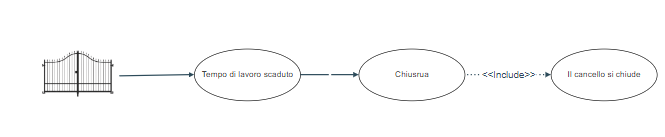
\includegraphics[width=0.8\textwidth]{use_case_us8.PNG}
    \caption{USE CASE user stories 8.}
    \label{fig:use_case_us5}
\end{figure}

\newpage
\subsubsection{Use Case generale}
In questo diagramma dei casi d'uso generale possiamo vedere tutte le azioni che l'utente può compiere per interagire con il sistema, così come le azioni automatiche del sistema che si attivano anche senza la presenza dell'utente.
\begin{figure}[h] % 'h' significa "here", posiziona l'immagine qui
    \centering % Centra l'immagine
    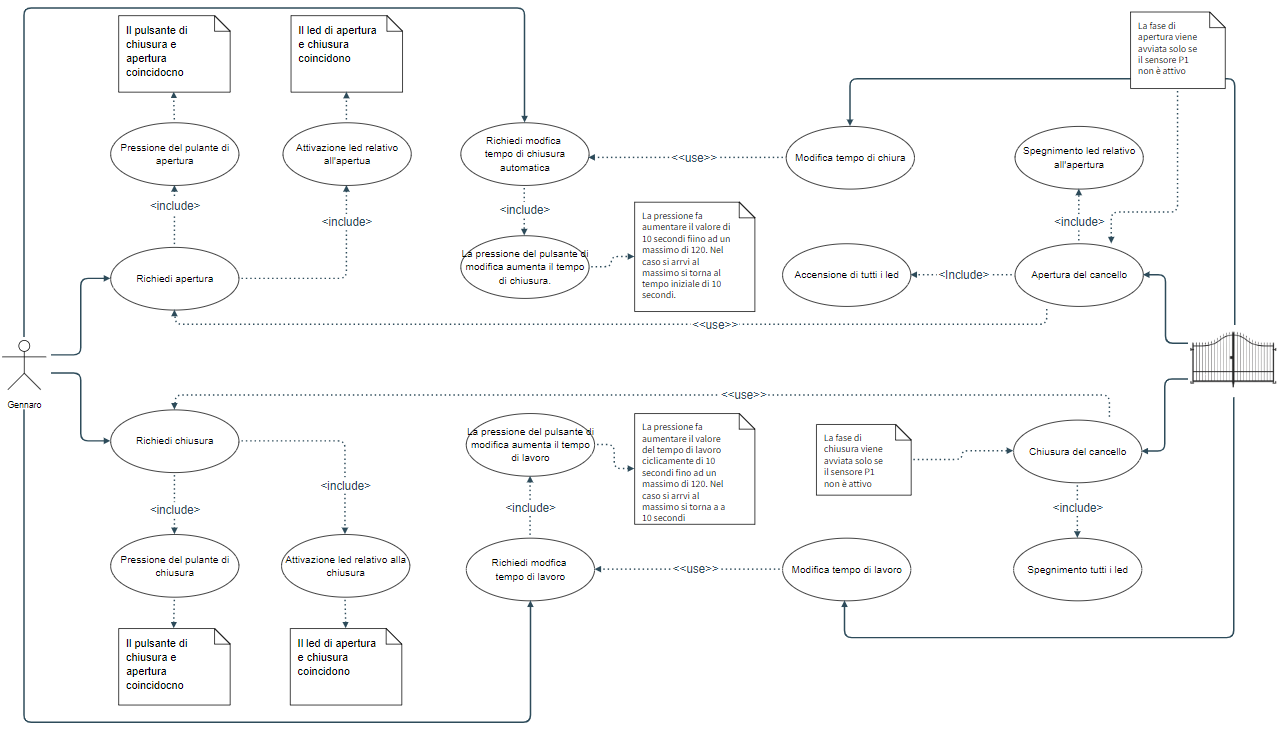
\includegraphics[width=1.1\textwidth, height=15cm, angle=270]{usa_case_diagram.PNG} % Inserisce l'immagine con una larghezza del 50% del testo
    \caption{Use case diagram} % Aggiunge una didascalia
    \label{fig:immagine} % Aggiunge un'etichetta per riferimenti incrociati
\end{figure}

\newpage
\subsection{Activity diagrams}
Testo dell'Activity diagram.
\subsubsection{Scenario 1}
Testo dello scenario 1
\subsubsection{Scenario 2}
Testo dello scenario 2
\subsubsection{Scenario 3}
Testo dello scenario 3
\subsubsection{Scenario 4}
Testo dello scenario 4
\subsubsection{Scenario 5}
Testo dello scenario 5
\subsubsection{Scenario 6}
Testo dello scenario 6
\subsubsection{Scenario 7}
Testo dello scenario 7

\subsection{State diagram}
Testo dello state diagram.

\section*{Elenco delle figure}
\addcontentsline{toc}{section}{Elenco delle figure}
\end{document}
